
\section{Representing power series}
\subsection{On the unit disc}
\begin{frame}
\frametitle{A practical representation for power series}
\begin{lemma}
Let $f : \C \to \C$ be analytic on the closed unit disc and $(a_m)_{m\in\N}$ its Taylor series around $0$.\\
Then $R>1$ \pause and we can find two positive integers $k$ and $A$ with 
\begin{itemize}
\item $r := \sqrt[k]{2}$ is strictly smaller than the radius of convergence $R$.
\item $|a_m|r^m \leq A$ for all $m \in \N$.
\end{itemize}
\end{lemma}
\pause
With $k$ and $A$ we can estimate 
$$ \left | \sum_{n \geq N} a_m z^n \right | \leq A\frac{(|z|/r)^N}{1-|z|/r} $$\pause
Consider triples $\big((a_m)_{n \in \N}, k, A\big)$ as representation for functions analytic on the unit disc.
\end{frame}
%\begin{frame}
%\frametitle{Finding $k$ and $A$}
%\begin{itemize}
%\item Choose $k$ appropriately and let $r := \sqrt{k}{2}$
%\item $f_{|z|=r}$ is a continuous function on a compact domain, thus is bounded by some number $A$
%\item By Cauchy Differentiation formula $$|a_n| \leq |\frac{1}{2\pi i}\int_{z=|r|} \frac{f(z)}{|z|^{n+1}} d \lambda| \leq \frac{A}{r^n}$$
%\end{itemize}
%\end{frame}
\begin{frame}[<+->]
\frametitle{Analytic Functions and Computational Complexity}
\begin{theorem}[Kawamura, R\"osnick, M\"uller, Ziegler (2013)]
  The following operators are computable in time polynomial in $k+log(A)+n$, where $2^{-n}$ is the output precision.
\begin{enumerate}
\item evaluation
\item addition and multiplication
\item differentiation and anti-differentiation
\item parametric maximization
\end{enumerate}
\end{theorem}
\end{frame}
\begin{frame}
\frametitle{But...}
\begin{center}
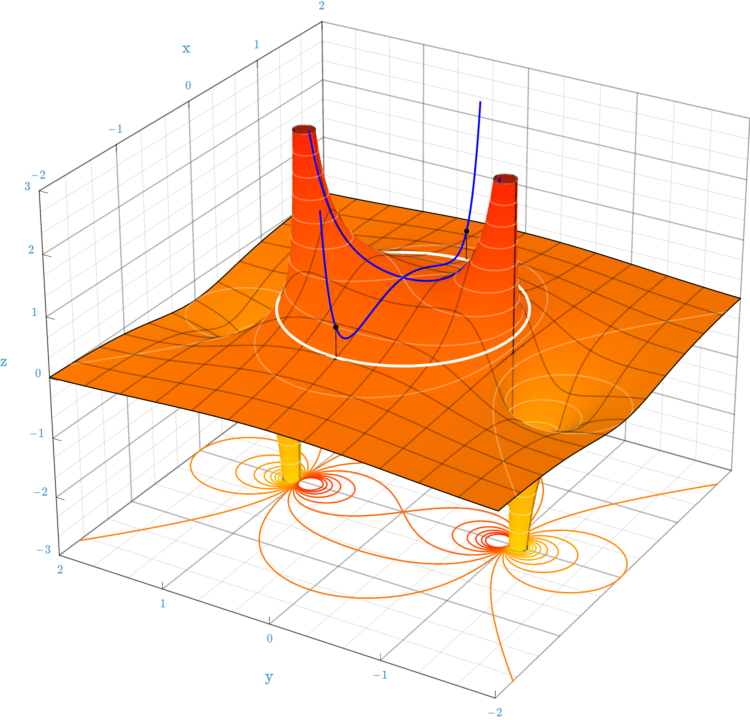
\includegraphics[width=0.6\textwidth]{TaylorComplexConv}
\end{center}
\end{frame}
\subsection{on $[-1,1]$}
\begin{frame}
\frametitle{\small Analytic functions on $[-1,1]$ (Kawamura, R\"osnick, M\"uller, Ziegler (2013))}
We want to consider complex functions analytic on $[-1,1]$.\\ 
\begin{minipage}{0.45\textwidth}
\begin{center}
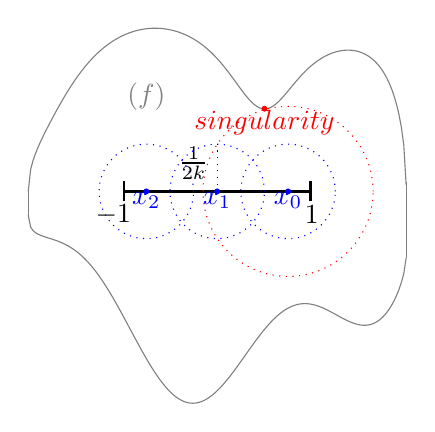
\begin{tikzpicture}[scale=0.6]
%    \draw<3> (-1,1) rectangle (5,-1);
    \node<1->  at (-0.2,-0.5) {$-1$};
    \node<1->  at (4.0,-0.5) {$1$};
    \draw<1-> [thick,|-|] (0,0) -- (4,0);
    \node<2>  at (1.5,.6) {$\frac 1{2k}$};
    \draw<2>  [dotted] (2.0,0) -- (2.0,1);
%    \node<3>  at (-.7,-.25) {$\frac 1l$};
%    \draw<3>  [dotted] (-1,0) -- (0,0);
%    \node<3>  at (2.2,.5) {$\frac 1l$};
%    \draw<3>  [dotted] (2,1) -- (2,0);
%    \node<3>  at (-.5,0.6) {$\overline R_l$};
    \draw<1-> [domain = 0:8,color=gray] plot[samples=160] (\x-2, {sqrt(16-(\x-4)^2)*(1-1/(\x^2+1) + sin(\x) + (\x/7)^5-\x/6 +1.5- 1/((\x-5)^2+1))/2});
    \draw<1-> [domain = 0:8,color=gray] plot[samples=160] (\x-2, {1/(\x^2+1)/2 + sin(80*\x) + (\x/7)^5-\x/6 -1-sqrt(16-(\x-4)^2)/2});
    \draw<1-> [color=gray] (-2,0) -- (-2,-.5);
    \draw<1-> [color=gray] (6,.19) -- (6,-1.42);
    \node<1-> [color=gray] at (.5,2) {$\dom(f)$};
    \draw<2> [fill=blue,radius =.05,color=blue] (3.5,0) circle;
    \node<2> [color=blue] at (3.5,-.2) {$x_0$};
    \draw<2> [fill=blue,radius =.05,color=blue] (2.0,0) circle;
    \node<2> [color=blue] at (2.0,-.2) {$x_1$};
    \draw<2> [radius = 1,color=blue, dotted] (2.0,0) circle; 
    \draw<2> [fill=blue,radius =.05,color=blue] (0.5,0) circle;
    \node<2> [color=blue] at (0.5,-.2) {$x_2$}; 
    \draw<2> [radius = 1,color=blue, dotted] (0.5,0) circle;
    \draw<2> [radius = 1,color=blue, dotted] (3.5,0) circle;
    \draw<2> [radius = 1.8, color = red, dotted] (3.5,0) circle; 
    \draw<1-> [fill=red,radius = .05,color = red] (3,1.75) circle;
    \node<1-> [color=red] at (3,1.45) {$singularity$};
    %\draw<3> [radius = 1, color = green, dotted] (2.5,0) circle;
    %\draw<3> [fill=green, radius = .05, color = green] (2.5,0) circle;
    %\node<3> [color=green] at (2.5,-.2) {$x_1$};
\end{tikzpicture}
\end{center}
\end{minipage}
\hfill
\begin{minipage}{0.45\textwidth}
\onslide<2->{
\begin{representation1}
  A finite number of taylor series together with parameters $A$ and $k$ that hold for each series, such that they cover the domain. 
 \end{representation1}
}
% \onslide<3->{
%\begin{representation2}
%A tuple $\big(f|_{[-1,1]}, B, l\big)$, $f \in C^\omega(\overline R_l)$ and $|f|_{\overline R_l}| \leq B$ where $\overline R_l := [-1-\frac1l,1+\frac1l]x[-\frac1l, \frac1l]$  
%\end{representation2}
%}
\end{minipage}
\end{frame}
%\begin{frame}
%\begin{minipage}{0.45\textwidth}
%\begin{representation1}
%A tuple $(M, (x_m), (a_{m,j}), A,k)$ $1 \leq m \leq M$, $j \in \N$ s.t. % with $1 \leq m \leq M$, $j \in \N$ so that
%%\item $a_{m,j}$ describes a Taylor series for $f$ around $x_m$ 
%$[-1,1] \subseteq \bigcup [x_m-\frac{1}{4k}, x_m+\frac{1}{4k}]$ \\
%and $|a_{m,j}| \leq A \cdot k^j$
% \end{representation1}
% \end{minipage}
% \hfill
% \begin{minipage}{0.45\textwidth}
%\begin{representation2}
%A tuple $\big(f|_{[-1,1]}, B, l\big)$, $f \in C^\omega(\overline R_l)$ and $|f|_{\overline R_l}| \leq B$ where $\overline R_l := [-1-\frac1l,1+\frac1l]x[-\frac1l, \frac1l]$  
%\end{representation2}
%\end{minipage}
%\begin{theorem}[Kawamura, R\"osnick, M\"uller, Ziegler (2013)]
%\begin{itemize}[<+->]
%\item Given $(M, (x_m), (a_{m,j}), A,k)$ we can evaluate $f(x)$ in time polynomial in $n+k+\lb(A)$
%\item From $(f,B,l)$ we can compute $(f^{(j)}(x_0))_{j \in \N}$ in time polynomial in $n+\lb(l)+\lb(B)$ 
%%and for all $x \in [-1,1]$ $|f^{(j)}(x)| \leq B\cdot l^j \cdot j!$
%\end{itemize}
%\end{theorem}
%\pause
%This means we can convert between those two representations in (parametrized) polynomial time.
%\end{frame} 

%\begin{frame}[<+->]
%\frametitle{Computing Taylor series}
%\begin{itemize}
%\item To convert between those representations we have to compute the Taylor coefficients from a given function
%\item Described in detail in (M\"uller87)
%\item Want to approximate the coefficient $a_m$ with max. error $2^{-n}$
%\item Approximate $f$ by Lagrangian interpolating polynomial $P_m(x) := \sum_{i=0}^{2m} f(x_i) \cdot L_{m,i}(x)$ with $L_{m,i}(x) = \prod_{j \neq i} \frac{x-x_j}{x_i-x_j} $ and $x_i = (i-m)\cdot h$
%\item Differentiate this polynomial $P^{(m)}(0) = \sum_{i=0}^{2m} f(z_i)\cdot L_{m,i}^{(m)}(0)$
%\item $\frac{1}{m!}P^{(m)}(0) = \sum_{i=0}^{2m} f(x_i)\frac{h^{-m}\cdot l_{m,i}}{i!(2m-i)!}$ with integers $l_{m,i}$
%\item An error bound for this approximation can be computed
%\end{itemize}
%\end{frame}


\begin{frame}
\frametitle{Evaluation}
\begin{minipage}{0.45\textwidth}

\begin{representation1}
  A finite number of taylor series together with parameters $A$ and $k$ that hold for each series covering the domain.
 \end{representation1}


\begin{representation2}
  A \textbf{single} taylor series together with parameters $A$ and $k$ that are valid for the the taylor series around any point of the domain.
\end{representation2}
\end{minipage}
\hfill
\begin{minipage}{0.45\textwidth}
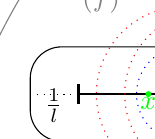
\begin{tikzpicture}[scale=0.6]
    \path [use as bounding box,red] (-30pt,-10pt) rectangle (30pt,40pt);
    \draw[rounded corners=4mm] (-1,1) rectangle (5,-1);
    %\draw (2,0) ellipse (3cm and 1cm);
    \draw [thick,|-|] (0,0) -- (4,0);
    \node at (-.5,-.25) {$\frac 1l$};
    \draw [dotted] (-1,0) -- (0,0);
    \node at (2.2,.5) {$\frac 1l$};
    \draw [dotted] (2,1) -- (2,0);
    \draw [domain = 0:8,color=gray] plot[samples=160] (\x-2, {sqrt(16-(\x-4)^2)*(1-1/(\x^2+1) + sin(\x) + (\x/7)^5-\x/6 +1.5- 1/((\x-5)^2+1))/2});
    \draw [domain = 0:8,color=gray] plot[samples=160] (\x-2, {1/(\x^2+1)/2 + sin(80*\x) + (\x/7)^5-\x/6 -1-sqrt(16-(\x-4)^2)/2});
    \draw [color=gray] (-2,0) -- (-2,-.5);
    \draw [color=gray] (6,.19) -- (6,-1.42);
    \node [color=gray] at (.5,2) {$\dom(f)$};
    \draw<1-3> [fill=blue,radius =.05,color=blue] (3.5,0) circle;
    \node<1-3> [color=blue] at (3.5,-.2) {$x_0$};
    \draw<1-3> [radius = 1,color=blue, dotted] (3.5,0) circle;
    \draw<1-3> [radius = 1.8, color = red, dotted] (3.5,0) circle; 
    \node<2> [color=red] at (2.5,-5) {Check if $x$ in circle};
    \draw [fill=green, radius = .05, color = green] (1.5,0) circle;
    \node [color=green] at (1.5,-.2) {$x$};
    \node<3> [color=red] at (3.0,-5) {Compute Taylor coefficients around $x_1$};
    \draw<3-5> [fill=cyan, radius = .05, color = cyan] (2.75,0) circle;
    \node<3-5> [color=cyan] at (2.75,-.2) {$x_1$};
    \draw<3-5> [radius = 1,color=cyan, dotted] (2.75,0) circle;
    \draw<4-5> [radius = 1.75, color = red, dotted] (2.75,0) circle; 
    \node<4> [color=red] at (2.5,-5) {Check if $x$ in circle};
    \node<5> [color=red] at (3.0,-5) {Compute Taylor coefficients around $x_2$};
    \draw<5-6> [fill=blue, radius = .05, color = blue] (2.25,0) circle;
    \node<5-6> [color=blue] at (2.25,-.2) {$x_2$};
    \draw<5-6> [radius = 1,color=blue, dotted] (2.25,0) circle;
    \draw<6> [radius = 1.85, color = red, dotted] (2.25,0) circle; 
\end{tikzpicture}
\end{minipage}
\end{frame}
